\textbf{Solution.}
\begin{enumerate}
  \item \textbf{ICE curves for $x_1$.}
  \begin{enumerate}
    \item Plugging in the values for $x_2$:
    \begin{align*}
      \hat f(x_1, 0) &= 3 - 8x_1 + 16x_1 \cdot 0 = 3 - 8x_1, \\
      \hat f(x_1, 1) &= 3 - 8x_1 + 16x_1 \cdot 1 = 3 - 8x_1 + 16x_1 = 3 + 8x_1.
    \end{align*}
    \item Both functions have intercept 3. The function for $x_2 = 0$ has slope $-8$ (decreasing), while the function for $x_2 = 1$ has slope $+8$ (increasing). They intersect at $x_1=0$ with value $3$. The slopes show a \emph{pure interaction}: the direction of effect of $x_1$ flips with $x_2$; no additive shift (same intercept 3).
  \end{enumerate}

  \item \textbf{Partial dependence of $x_1$.}
  \begin{enumerate}
    \item Using the hint, we average over $X_2$:
    \begin{align*}
      \mathrm{PD}_{x_1}(t) &= \E_{X_2}[\hat f(t,X_2)] \\
      &= \Pr(x_2=0) \cdot \hat f(t,0) + \Pr(x_2=1) \cdot \hat f(t,1) \\
      &= 0.5 \cdot (3 - 8t) + 0.5 \cdot (3 + 8t) \\
      &= 0.5(3 - 8t) + 0.5(3 + 8t) \\
      &= 1.5 - 4t + 1.5 + 4t = 3.
    \end{align*}
    \item The partial dependence function is constant at 3. The sketch shows:
    \begin{figure}[h!]
      \centering
      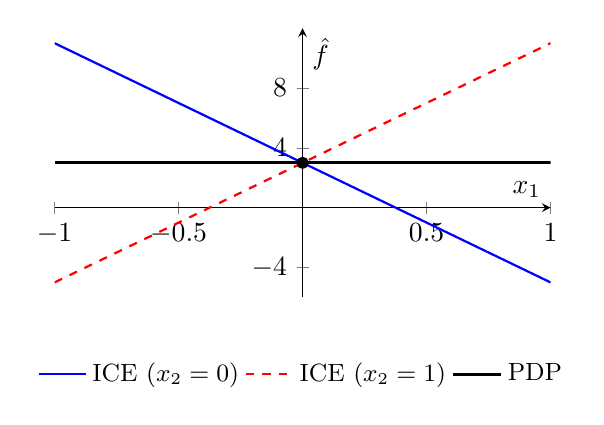
\begin{tikzpicture}
        \begin{axis}[
          width=0.65\textwidth,
          height=5.0cm,
          xmin=-1, xmax=1,
          ymin=-6, ymax=12,
          axis lines=middle,
          xlabel={$x_1$}, ylabel={$\hat f$},
          xtick={-1,-0.5,0,0.5,1},
          ytick={-8,-4,0,4,8},
          samples=101,
          domain=-1:1,
          legend style={draw=none,at={(0.5,-0.2)},anchor=north,legend columns=3,font=\small}
        ]
          \addplot[blue, thick] {-8*x + 3}; \addlegendentry{ICE ($x_2=0$)}
          \addplot[red, thick, dashed] {8*x + 3}; \addlegendentry{ICE ($x_2=1$)}
          \addplot[black, very thick] {3}; \addlegendentry{PDP}
          \addplot[only marks, mark=*, mark size=2pt] coordinates {(0,3)};
        \end{axis}
      \end{tikzpicture}
    \end{figure}
    \item The partial dependence is flat at 3 because the opposite slopes ($-8$ and $+8$) cancel out when averaged. This hides the strong conditional effects visible in the ICE curves. The ICE curves show that $x_1$ has a strong effect in opposite directions depending on $x_2$, but the PDP suggests no effect. This demonstrates why inspecting ICE curves (or ICE variance) is critical to avoid concluding ``no effect'' when interactions are present.
  \end{enumerate}
\end{enumerate}

